\documentclass[12pt]{article}
\usepackage{graphicx} % Required for inserting images
\usepackage{enumitem}
\usepackage{amsmath}
\usepackage{gvv-book}
\usepackage{gvv}

\title{\textbf{4.2.7}}
\author{\textbf{EE25BTECH11004 - Aditya Appana}}
\date{September 9, 2025}

\begin{document}

\maketitle

\section*{Question}
Find the direction and normal vectors of the line $y-2=0$

\section*{Solution}
A line can be expressed in two forms:
\begin{align}
\myvec{x\\y} = \myvec{0\\c} + x\myvec{1\\m}
\end{align}
where \myvec{1\\m} is the direction vector of the line and m is the \textbf{slope} of the line.

\begin{align}
{\vec{n}}^{T}x = c
\end{align}
where $\vec{n}$ is the normal vector of the line. \begin{align}{\vec{n}}^T\myvec{1\\m} = 0\end{align}

\vspace{1cm}

The slope of the line $y-2=0$ is 0, therefore it can be expressed in the first form as:
\begin{align}
\myvec{x\\y} = \myvec{0\\2} + x\myvec{1\\0}
\end{align}\\

Let \myvec{x\\y} be normal vector. Therefore
\begin{align}
\myvec{x\\ y}^T\myvec{1\\0} = 0 \\
x = 0\\
\myvec{x\\y} = \myvec{0\\1}
\end{align}

Therefore the line can be expressed as

\begin{align}
\myvec{0\\1}^Tx=2
\end{align}

\vspace{1cm}


Therefore, the direction vector is \myvec{1\\0} , and the normal vector is \myvec{0\\1}.



\begin{figure}[H]
    \centering
    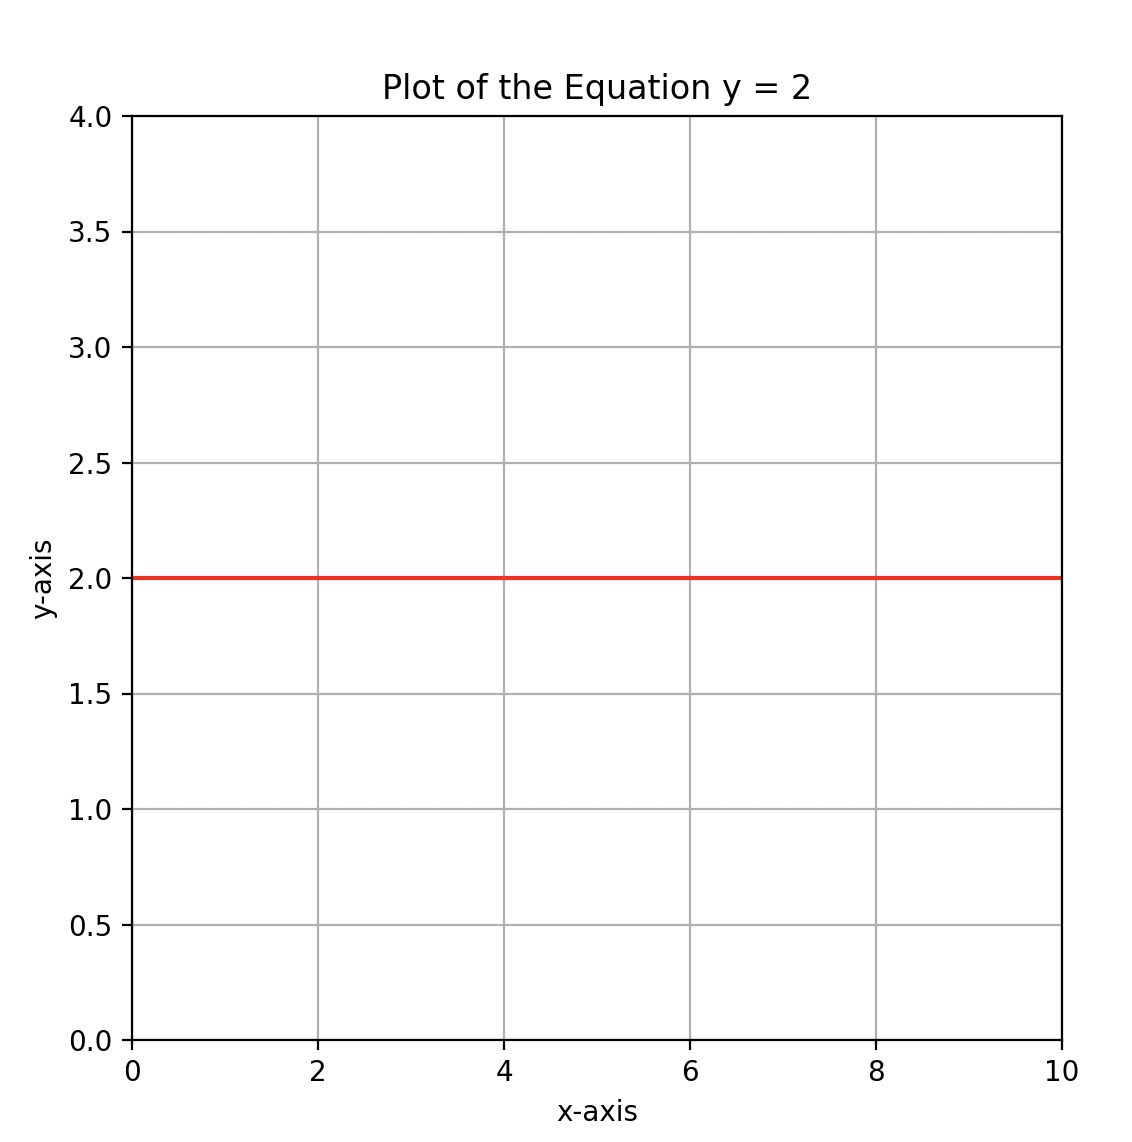
\includegraphics[width=0.7\columnwidth]{Figs/Y=2.png}
    \caption{Equilateral Triangle}
    \label{fig:placeholder}
\end{figure}

\end{document}